\begin{figure}[htbp]
\centering
\begin{minipage}[t]{.47\linewidth}
\centering
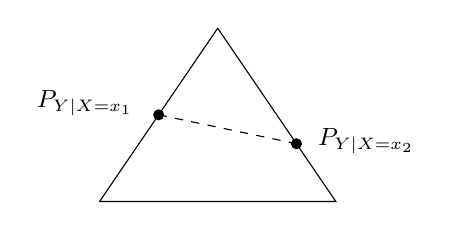
\begin{tikzpicture}[x=1cm,y=1cm]
 \draw (0,0)--(1.5,2.2)--(3,0)--cycle;
 \draw[dashed] (.75,1.1)--(2.5,.733333);
 \fill (.75,1.1) circle[radius=2pt];
 \fill (2.5,.733333) circle[radius=2pt];
 \node[left,font=\small] at (.55,1.25) {$P_{Y\mid X=x_1}$};
 \node[right,font=\small] at (2.65,.77) {$P_{Y\mid X=x_2}$};
\end{tikzpicture}
\par\small (a) 纯条件分布的示例：延长连接$P_{Y\mid X=x_1}$与$P_{Y\mid X=x_2}$的线段，就会离开概率分布单纯形。
\end{minipage}\hfill
\begin{minipage}[t]{.47\linewidth}
\centering
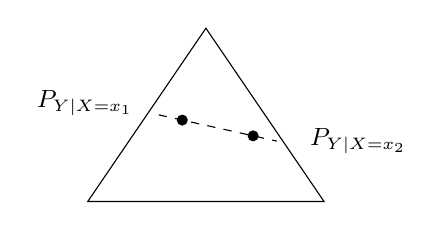
\begin{tikzpicture}[x=1cm,y=1cm]
 \draw (0,0)--(1.5,2.2)--(3,0)--cycle;
 \draw[dashed] (.9,1.1)--(2.4,.766667);
 \fill (1.2,1.033333) circle[radius=2pt];
 \fill (2.1,.833333) circle[radius=2pt];
 \node[left,font=\small] at (.7,1.25) {$P_{Y\mid X=x_1}$};
 \node[right,font=\small] at (2.7,.77) {$P_{Y\mid X=x_2}$};
\end{tikzpicture}
\par\small (b) 非纯条件分布的示例：连接$P_{Y\mid X=x_1}$与$P_{Y\mid X=x_2}$的线段，可以稍作延长而不离开单纯形。
\end{minipage}
\caption{纯条件分布与非纯条件分布的可视化。}
\end{figure}
